\documentclass[conference]{IEEEtran}
\IEEEoverridecommandlockouts
% The preceding line is only needed to identify funding in the first footnote. If that is unneeded, please comment it out.
\usepackage{cite}
\usepackage[spanish]{babel}
\usepackage{amsmath,amssymb,amsfonts}
\usepackage{algorithmic}
\usepackage{graphicx}
\usepackage{textcomp}
\usepackage{xcolor}
\usepackage{listings}
\usepackage{caption}
\usepackage{subcaption}
\setlength{\parskip}{12pt}
\usepackage[numbers]{natbib}
%\renewcommand{\refname}{Referencias}
\def\BibTeX{{\rm B\kern-.05em{\sc i\kern-.025em b}\kern-.08em
    T\kern-.1667em\lower.7ex\hbox{E}\kern-.125emX}}
\renewcommand{\lstlistingname}{Programa}
\definecolor{codegreen}{rgb}{0,0.6,0}
\definecolor{codegray}{rgb}{0.5,0.5,0.5}
\definecolor{codepurple}{rgb}{0.58,0,0.82}
\definecolor{backcolour}{rgb}{0.95,0.95,0.92}

\lstdefinestyle{mystyle}{
	backgroundcolor=\color{backcolour},   
	commentstyle=\color{codegreen},
	keywordstyle=\color{magenta},
	numberstyle=\tiny\color{codegray},
	stringstyle=\color{codepurple},
	basicstyle=\ttfamily\footnotesize,
	breakatwhitespace=false,         
	breaklines=true,                 
	captionpos=b,                    
	keepspaces=true,                 
	numbers=left,                    
	numbersep=5pt,                  
	showspaces=false,                
	showstringspaces=false,
	showtabs=false,                  
	tabsize=2
}
\lstset{style=mystyle}
\begin{document}

\title{Integración de memristores en redes neuronales artificiales para la clasificación del conjunto de datos MNIST utilizando TensorFlow\\
%{\footnotesize \textsuperscript{*}Note: Sub-titles are not captured in Xplore and should not be used}
%\thanks{Identify applicable funding agency here. If none, delete this.}
}

\author{\IEEEauthorblockN{1\textsuperscript{st} Ricardo Aldair Tirado Torres}
\IEEEauthorblockA{\textit{Centro de Investigación en Computación} \\
\textit{Instituto Politécnico Nacional}\\
Ciudad de México, México \\
rtiradot2023@cic.ipn.mx}
\and
\IEEEauthorblockN{2\textsuperscript{nd} Ricardo Barrón Fernández}
\IEEEauthorblockA{\textit{Centro de Investigación en Computación} \\
	\textit{Instituto Politécnico Nacional}\\
	Ciudad de México, México \\
	rbarron@cic.ipn.mx}
}
\maketitle

\begin{abstract}
El cómputo neuromórfico, con sus redes neuronales pulsantes, el aprendizaje STDP y los memristores, representa un paradigma revolucionario en la informática. La integración de estos conceptos en la tecnología CMOS no solo promete un salto significativo en la eficiencia y capacidad de las máquinas, sino que también nos acerca un paso más a replicar la asombrosa complejidad y eficiencia del cerebro humano. Esta tecnología abre un abanico de posibilidades en el campo de la inteligencia artificial y más allá, con el potencial de transformar la forma en que interactuamos con las máquinas y el mundo que nos rodea. En este trabajo se utiliza al nodo tecnológico de SKY130, un proceso de fabricación que integra los elementos necesarios para diseñar una red neuronal pulsante que integra el concepto del aprendizaje STDP no supervisado.
\end{abstract}

\begin{IEEEkeywords}
Redes neuronales artificiales, sinapsis memristiva, clasificación de patrones, memristor HP.
\end{IEEEkeywords}

\section{Introducción}
Las redes neuronales artificiales (ANNs, por sus siglas en inglés) son modelos computacionales inspirados en la estructura y el funcionamiento del cerebro humano, diseñados para realizar tareas de reconocimiento de patrones, clasificación y predicción. Estas redes consisten en capas de neuronas artificiales conectadas entre sí, donde cada conexión tiene un peso asociado que se ajusta durante el proceso de entrenamiento. \cite{mem1} El entrenamiento de una ANN implica la optimización de estos pesos mediante algoritmos de aprendizaje, siendo el descenso de gradiente uno de los métodos más comunes. Una vez entrenada, la red puede realizar inferencias sobre datos nuevos, aplicando los pesos optimizados para generar predicciones o clasificaciones. \cite{mem2}

En el ámbito de la inteligencia artificial, las ANNs se utilizan extensamente para la clasificación de patrones \cite{mem3} \cite{mem4}, un proceso crucial en aplicaciones como el reconocimiento de imágenes, el procesamiento del lenguaje natural y la detección de fraudes. El aprendizaje profundo, una subrama del aprendizaje automático que se basa en ANNs con múltiples capas (redes neuronales profundas), ha revolucionado estos campos, logrando avances significativos en precisión y eficiencia.

Los memristores han emergido como una tecnología prometedora para implementar pesos sinápticos en redes neuronales artificiales. Un memristor es un componente electrónico cuya resistencia puede ser ajustada y memorizada, comportándose de manera análoga a una sinapsis biológica. \cite{mem5} En el contexto del aprendizaje máquina y el aprendizaje profundo, los memristores ofrecen una solución eficiente para el almacenamiento y ajuste de pesos sinápticos, permitiendo la creación de hardware neuromórfico que puede ejecutar tareas de inferencia y entrenamiento de manera más rápida y con menor consumo de energía en comparación con los sistemas tradicionales basados en transistores. \cite{mem6}

El memristor de HP, desarrollado por Hewlett-Packard \cite{HP}, es uno de los primeros y más conocidos dispositivos de este tipo, capaz de recordar su estado resistivo incluso después de apagar la energía. Este atributo lo hace ideal para su uso en ANNs, donde puede representar y ajustar eficientemente los pesos sinápticos, facilitando así la implementación de redes neuronales en dispositivos de hardware especializados. 

Para evaluar y entrenar redes neuronales, se utilizan conjuntos de datos estandarizados que permiten medir el rendimiento y la precisión del modelo. \cite{mem7} \cite{mem8}Uno de los conjuntos de datos más utilizados en la investigación de ANNs es el MNIST (\textit{Modified National Institute of Standards and Technology}), que contiene 60,000 imágenes de entrenamiento y 10,000 imágenes de prueba de dígitos escritos a mano, cada una con una resolución de 28x28 píxeles. Este conjunto de datos ha sido fundamental para el desarrollo y \textit{benchmarking} de nuevas arquitecturas de redes neuronales y técnicas de aprendizaje automático. \cite{mem9} \cite{mem10}

Este reporte explorará en detalle los conceptos mencionados, comenzando con una revisión de las redes neuronales artificiales, seguido de una discusión sobre el papel de los memristores como pesos sinápticos, destacando el memristor de HP, y finalizando con la descripción de arquitectura de la red neuronal diseñada con la herramienta TensorFlow, evaluando el desempeño de nuestro modelo en la tarea de clasificación de imágenes.

\begin{figure}[ht]
	\centering
	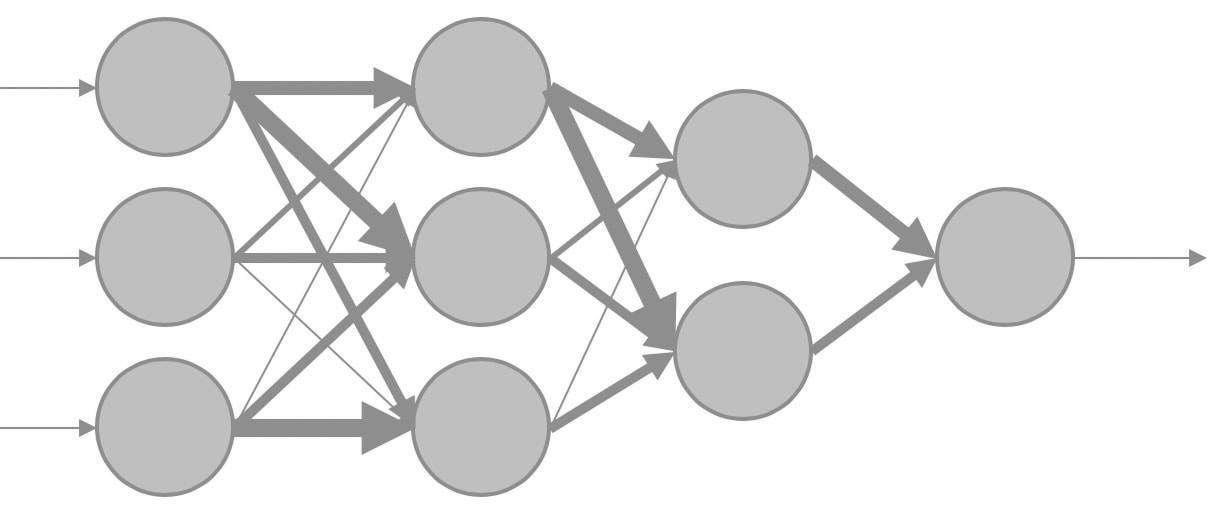
\includegraphics[scale=0.2]{img/ANN.png}
	\caption{Diagrama de una red neuronal artificial con las diferentes capas interconectadas.
		\label{fig:ann}}
\end{figure}

\section{Preliminares}

\subsection{Redes neuronales artificiales}
Las redes neuronales artificiales (ver Figura \ref{fig:ann}) son modelos computacionales inspirados en la estructura y el funcionamiento del cerebro humano. \cite{mem11} Estas redes están compuestas por unidades interconectadas llamadas neuronas artificiales, distribuidas típicamente en tres tipos de capas:

\begin{itemize}
	\item \textit{Capa de entrada}: Recibe las señales iniciales del entorno externo. En el caso de la clasificación de imágenes, cada neurona de la capa de entrada representa un píxel de la imagen.
	\item \textit{Capas ocultas}: Procesan las señales de entrada mediante una serie de transformaciones no lineales. Estas capas están compuestas por neuronas que aplican funciones de activación a sus entradas ponderadas.
	\item \textit{Capa de salida}: Genera la salida final del modelo. Para la clasificación, cada neurona en la capa de salida puede representar una clase diferente.
\end{itemize}

\begin{figure}[ht]
	\centering
	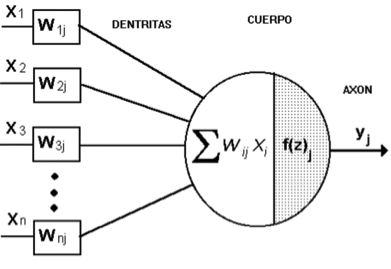
\includegraphics[scale=0.55]{img/Neuron.png}
	\caption{Esquema de una neurona artificial.
		\label{fig:neuron}}
\end{figure}

Como se visualiza en la Figura \ref{fig:neuron}, cada neurona en una red neuronal artificial realiza una operación matemática sobre sus entradas ponderadas y una función de activación. La salida de una neurona $j$ se puede representar matemáticamente como:

\begin{equation}
	y_{j} = f(z)_{j} \left( \sum_{i}^{n} w_{ij}x_{i} + b_{i} \right)
	\label{eq:1}
\end{equation}

Donde:

\begin{itemize}
	\item $y_{j}$ es la salida de la neurona .
	\item $f(z)_{j}$ es la función de activación (por ejemplo, ReLU, sigmoide, tanh).
	\item $w_{ij}$ es el peso sináptico entre la neurona $i$ de la capa anterior y la neurona $j$.
	\item $x_{i}$ es la entrada desde la neurona $i$ de la capa anterior.
	\item $b_{j}$ es el sesgo de la neurona $j$
\end{itemize}

El proceso de entrenamiento de una red neuronal implica ajustar los pesos sinápticos $w_{ij}$ y los sesgos $b_{j}$ para minimizar una función de pérdida, que mide la diferencia entre las predicciones de la red y los valores reales. Este ajuste se realiza mediante un algoritmo de optimización, junto con un proceso de retropropagación del error.

Existen varios tipos de redes neuronales artificiales, siendo las redes neuronales \textit{feedforward} o FFNN, uno de los tipos más simples y ampliamente utilizados. \cite{mem12} En una FFNN, las conexiones entre las unidades no forman ciclos, y la información fluye solo en una dirección: desde las capas de entrada, a través de las capas ocultas, y finalmente hacia la capa de salida. El funcionamiento de este tipo de red neuronal se puede describir de la siguiente manera:

\begin{itemize}
	\item \textit{Propagación hacia Adelante:} Las entradas se pasan a través de la capa de entrada. Las salidas de cada neurona de la capa de entrada se multiplican por los pesos correspondientes y se pasan a las neuronas de la primera capa oculta. Cada neurona de la capa oculta suma sus entradas ponderadas y aplica una función de activación para calcular su salida.	Este proceso se repite para todas las capas ocultas hasta llegar a la capa de salida.	La capa de salida produce la predicción final del modelo.
	\item \textit{Cálculo de la Pérdida:} La salida de la red se compara con la etiqueta verdadera utilizando una función de pérdida (como la entropía cruzada esparsa para problemas de clasificación). La función de pérdida cuantifica la discrepancia entre la predicción del modelo y el valor verdadero.
	\item \textit{Retropropagación del Error:} El error calculado se propaga hacia atrás a través de la red. Se calculan los gradientes de la función de pérdida respecto a los pesos y sesgos utilizando el algoritmo de retropropagación. Estos gradientes indican la dirección y magnitud en la que deben ajustarse los pesos para reducir la pérdida. 
	\item \textit{Actualización de Pesos:} Los pesos y sesgos se actualizan utilizando un algoritmo de optimización, como el gradiente descendente o una de sus variantes. La actualización de los pesos se realiza para minimizar la función de pérdida y mejorar la precisión del modelo.
\end{itemize}

Las ventajas de utilizar FFNN es que son las redes neuronales más simples de entender y implementar en comparación con otros tipos de redes neuronales, son adecuadas para una amplia variedad de tareas de predicción y clasificación y requieren menos recursos computacionales en comparación con redes más complejas como las redes convolucionales (CNN) y las redes recurrentes (RNN). No obstante, tienen limitaciones en el procesamiento de datos espaciales y temporales ya que no capturan bien las relaciones espaciales en datos como imágenes (para lo cual se utilizan las CNN) o las dependencias temporales en series de tiempo (para lo cual se utilizan las RNN). De igual forma, en redes profundas, las FFNN pueden sufrir de problemas de \textit{vanishing gradients} (gradientes que se desvanecen), lo que dificulta el entrenamiento de capas muy profundas. \cite{mem13}

\subsection{Memristores}
Los memristores (resistores de memoria) son componentes eléctricos pasivos que han sido teorizados durante décadas y que finalmente se desarrollaron experimentalmente en los últimos años. Estos dispositivos se caracterizan por su capacidad para recordar la cantidad de carga que ha pasado a través de ellos, lo que les permite retener un estado resistivo específico incluso después de que se ha eliminado la fuente de energía. Esta propiedad de memoria los hace especialmente adecuados para aplicaciones en almacenamiento de datos no volátil y procesamiento neuromórfico. \cite{HP1}

La idea de los memristores fue propuesta por primera vez por Leon Chua en 1971. \cite{Chua_1971} Chua predijo la existencia de un cuarto elemento pasivo fundamental en los circuitos eléctricos, junto con el resistor, el capacitor y el inductor. Este cuarto elemento, el memristor, tiene una relación directa entre el flujo magnético y la carga eléctrica, lo que le confiere sus propiedades únicas. El memristor se define matemáticamente por la ecuación \ref{eq:2} y \ref{eq:3}.

\begin{equation}
	V = R(w) \cdot I
	\label{eq:2}
\end{equation}

\begin{equation}
	\frac{dw}{dt} = f(I)
	\label{eq:3}
\end{equation}

Donde:
\begin{itemize}
	\item $V$ es la tensión a través del memristor.
	\item $I$ es la corriente que pasa a través del memristor.
	\item $R(w)$ es la resistencia dependiente del estado $\omega$, que es una función de la carga histórica.
\end{itemize}

\begin{figure}[ht]
	\centering
	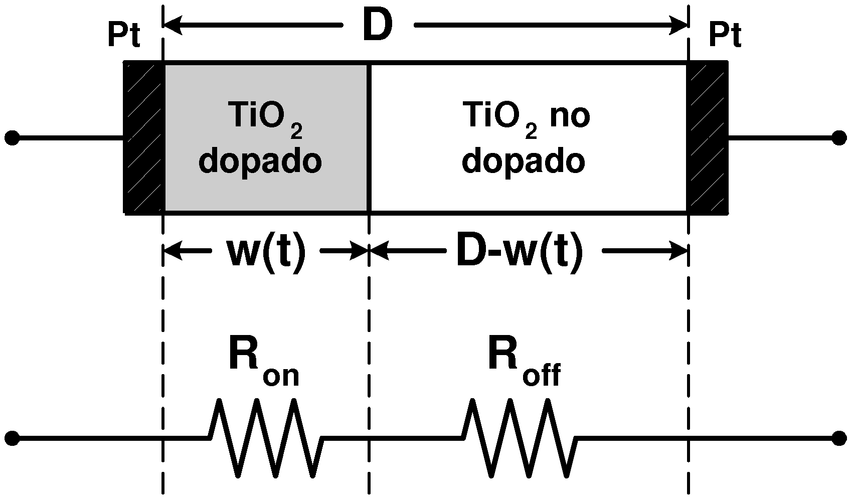
\includegraphics[scale=0.27]{img/MemristorHP.png}
	\caption{Estructura física del memristor sintetizado por HP Labs.
		\label{fig:memristorhp}}
\end{figure}

Las características principales de este componente eléctrico es la capacidad de retener un estado resistivo específico sin necesidad de energía continua, esto a su vez genera una analogía con las sinapsis, ya que su comportamiento es similar al de las sinapsis neuronales, donde la resistencia del memristor puede ajustarse de manera análoga a la fuerza sináptica en las redes biológicas. Además de lo anteriormente descrito, los memristores ofrecen alta densidad de almacenamiento y baja energía de operación en comparación con los dispositivos convencionales.

\subsection{Memristor de HP}
En 2008, un equipo de investigadores de HP Labs, dirigido por Stanley Williams, fabricó el primer memristor funcional utilizando una estructura de óxido de metal. \cite{HP2} Este desarrollo confirmó la existencia de los memristores y abrió nuevas posibilidades para su uso en la tecnología de la información.

El memristor de HP (ver Figura \ref{fig:memristorhp}) se construye con una película delgada de dióxido de titanio ($TiO_{2}$) colocada entre dos electrodos de platino. La película de $TiO_{2}$ tiene dos capas: una capa de $TiO_{2}$ pura y otra con oxígeno deficitario ($TiO_{2-x}$). La migración de los vacantes de oxígeno entre estas capas, causada por una corriente eléctrica, modifica la resistencia del dispositivo. \cite{HP3}

\begin{itemize}
	\item Estado de Alta Resistencia (HRS): Cuando los vacantes de oxígeno están distribuidos uniformemente, el memristor está en un estado de alta resistencia.
	\item Estado de Baja Resistencia (LRS): Cuando una corriente eléctrica hace que los vacantes de oxígeno se acumulen en la capa de $TiO_{2-x}$, el dispositivo entra en un estado de baja resistencia.
\end{itemize}

El modelo de HP se puede describir con las ecuaciones diferenciales que rigen la dinámica del dispositivo, vistas en la ecuación \ref{eq:4} y \ref{eq:5}:

\begin{equation}
	R(w) = R_{on} \cdot w + R_{off} \cdot (1 - w)
	\label{eq:4}
\end{equation}

\begin{equation}
	\frac{dw}{dt} = \mu \cdot \frac{I}{D}
	\label{eq:5}
\end{equation}

Donde:
\begin{itemize}
	\item $R_{on}$ y $R_{off}$ son las resistencias mínima y máxima del memristor.
	\item $w$ es una variable de estado que representa la proporción de la capa de $TiO_{2}$ dopada.
	\item $\mu$ es la movilidad de los vacantes de oxígeno.
	\item $D$ es el espesor de la película de $TiO_{2}$.
\end{itemize}

Los memristores tienen aplicaciones potenciales en varias áreas, como el almacenamiento de datos puesto que pueden reemplazar a la memoria flash debido a su alta densidad y velocidad, también pueden ser usados en circuitos lógicos reconfigurables, proporcionando una alternativa flexible y eficiente en términos energéticos a los transistores tradicionales. Actualmente el campo en el que los memristores tienen un futuro muy prometedor es en el cómputo neuromórfico, debido a que la integración de memristores en redes neuronales artificiales ofrece una solución prometedora para mejorar la eficiencia energética y la densidad de almacenamiento de estos sistemas. Los memristores pueden emular las sinapsis biológicas al proporcionar una forma no volátil y analógica de almacenamiento y procesamiento de información, alineando el hardware de computación más estrechamente con la estructura y el funcionamiento del cerebro humano. En la siguiente sección, describimos nuestro enfoque para integrar un modelo de memristor de HP en una red neuronal artificial para la clasificación del conjunto de datos MNIST, utilizando TensorFlow.

\section{Sistema propuesto}

El sistema propuesto integra un modelo de memristor de HP en una red neuronal artificial para la clasificación del conjunto de datos MNIST utilizando la herramienta TensorFlow. Este enfoque busca aprovechar las propiedades únicas de los memristores para mejorar la eficiencia energética y la capacidad de almacenamiento del sistema de aprendizaje automático. A continuación, se detalla la arquitectura de la red neuronal, el funcionamiento del programa, el modelo de memristor utilizado y el algoritmo de entrenamiento.

\subsection{Arquitectura de la Red Neuronal}
La red neuronal utilizada en este trabajo es una red neuronal \textit{feedforward} (FFNN) con las siguientes características:

\begin{itemize}
	\item \textit{Capa de Entrada:} Una capa que toma imágenes de 28x28 píxeles del conjunto de datos MNIST, aplanando cada imagen en un vector de 784 dimensiones.
	\item \textit{Capa Oculta Personalizada con Memristores:} Una capa que simula el comportamiento de un memristor de HP, con 128 unidades (neuronas).
	\item \textit{Capa de Activación:} Una capa de activación ReLU (\textit{Rectified Linear Unit}) que introduce no linealidad en el modelo.
	\item \textit{Capa de Salida:} Una capa densa (completamente conectada) con 10 neuronas, cada una correspondiente a una de las 10 clases de dígitos (0-9) del conjunto de datos MNIST.
\end{itemize}

El modelo de memristor de HP se integra en la capa oculta personalizada. La actualización de los pesos sinápticos en esta capa se realiza mediante una ecuación diferencial simplificada que describe la dinámica de los memristores, previamente descrita.

El programa se implementa en Python utilizando TensorFlow, una biblioteca de código abierto para la construcción y entrenamiento de modelos de aprendizaje profundo. El flujo de trabajo del programa es el siguiente:

\begin{enumerate}
	\item \textit{Carga y Preprocesamiento de Datos:} Se carga el conjunto de datos MNIST y se normalizan las imágenes dividiendo los valores de los píxeles por 255 para que los valores estén en el rango [0, 1].
	\item \textit{Definición de la Capa Personalizada:} Se define una capa personalizada que simula el comportamiento del memristor de HP. Esta capa realiza la actualización de los pesos sinápticos en función de la corriente que pasa a través de ellos.
	\item \textit{Construcción del Modelo:} Se construye el modelo de la red neuronal utilizando la capa personalizada junto con capas adicionales de activación y salida.
	\item \textit{Compilación del Modelo:} Se compila el modelo utilizando el optimizador \textit{Adam} y la función de pérdida de entropía cruzada esparsa para la clasificación.
	\item \textit{Entrenamiento del Modelo:} Se entrena el modelo durante varias épocas en el conjunto de entrenamiento de MNIST.
	\item \textit{Evaluación del Modelo:} Se evalúa el modelo en el conjunto de prueba de MNIST para determinar su precisión.
	\item \textit{Predicción y Visualización:} Se realizan predicciones en el conjunto de prueba y se visualizan algunas de las predicciones junto con sus etiquetas verdaderas.
\end{enumerate}

El algoritmo de entrenamiento utilizado es el gradiente descendente, implementado mediante el optimizador \textit{Adam}. Este algoritmo ajusta los pesos sinápticos para minimizar la función de pérdida. Los pasos del algoritmo son los siguientes:

\begin{enumerate}
	\item Los pesos y sesgos de la red se inicializan aleatoriamente.
	\item Los datos de entrada se propagan a través de la red para generar predicciones.
	\item Se calcula la función de pérdida que mide la discrepancia entre las predicciones y las etiquetas verdaderas.
	\item El error se propaga hacia atrás a través de la red para calcular los gradientes de la función de pérdida respecto a los pesos y sesgos.
	\item Los pesos y sesgos se actualizan utilizando los gradientes calculados y el algoritmo de optimización \textit{Adam}.
\end{enumerate}

\section{Resultados}

\begin{figure}[ht]
	\centering
	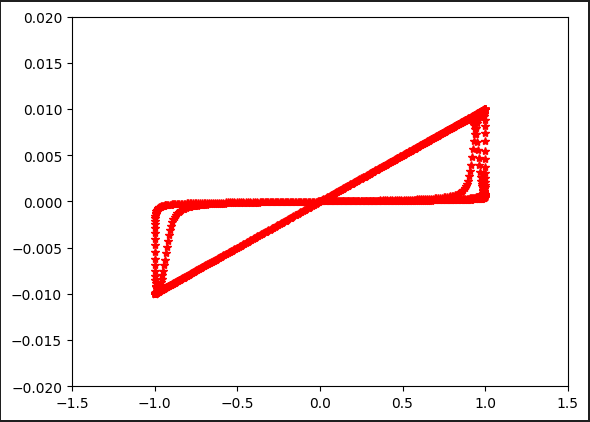
\includegraphics[scale=0.55]{img/Histeresis.png}
	\caption{Ciclo de histéresis del memristor de HP.
		\label{fig:histeresis}}
\end{figure}

\begin{figure}[ht]
	\centering
	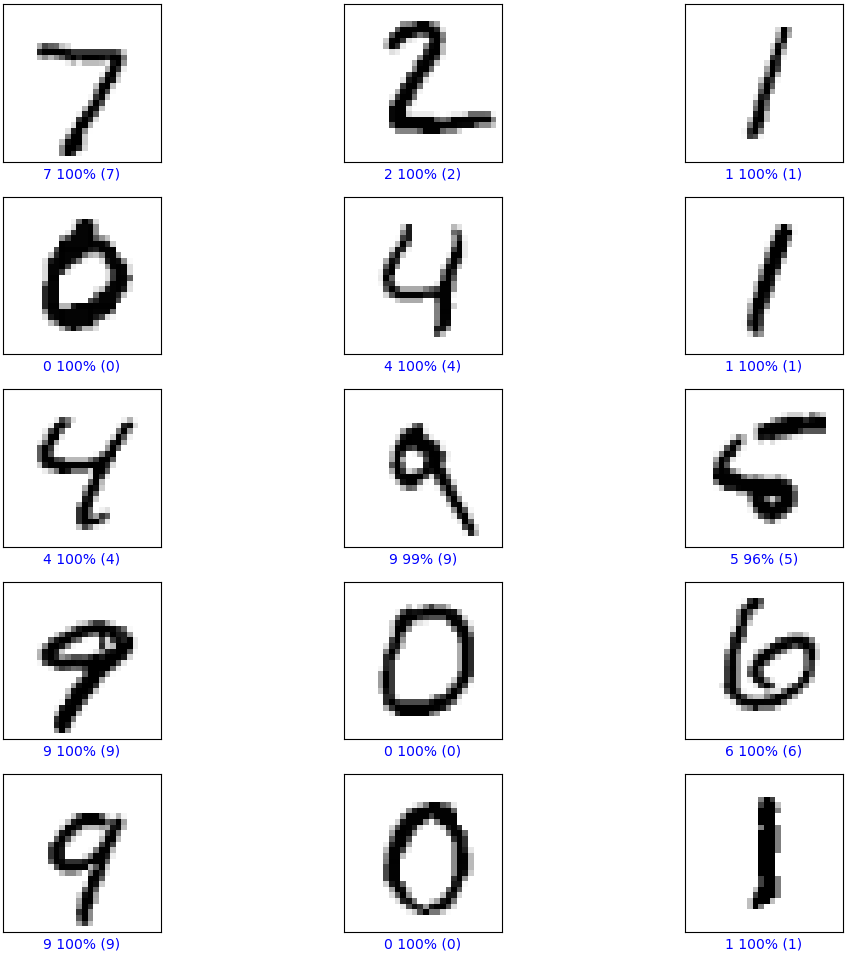
\includegraphics[scale=0.29]{img/Resultados.png}
	\caption{Predicciones realizadas por el modelo.
		\label{fig:resultados}}
\end{figure}

En la Figura \ref{fig:histeresis} se observa el ciclo de histéresis del modelo de memristor utilizado. Se aprecia el fenómeno de \textit{snapback} que se refiere a una disminución repentina y pronunciada en la resistencia del dispositivo cuando se aplica una determinada tensión. En términos de una curva I-V (corriente versus voltaje), el \textit{snapback} se manifiesta como un cambio abrupto en la corriente para un pequeño cambio en el voltaje, seguido de una disminución en la resistencia.

Con respecto al entrenamiento de la red neuronal, se muestra en el Cuadro \ref{tab:entrenamiento} el resultado de entrenar la red en 5 épocas, obteniéndose una precisión en la prueba de clasificación del $97.89\%$. En la Figura \ref{fig:resultados} se muestran algunas de las imágenes clasificadas y la precisión de la red ante esa instancia.

\begin{table}[htbp]
\caption{Entrenamiento de la red neuronal}
\begin{center}
\begin{tabular}{|c|c|c|}
\hline
\cline{1-3} 
\textbf{\textit{Época}} & \textbf{\textit{Precisión}}& \textbf{\textit{Pérdida}} \\
\hline
$1$ & $88.14\%$ & $42.9\%$ \\
\hline
$2$ & $96.49\%$ & $12\%$ \\
\hline
$3$ & $97.66\%$ & $7.85\%$ \\
\hline
$4$ & $98.29\%$ & $5.78\%$ \\
\hline
$5$ & $98.63\%$ & $4.4\%$ \\
\hline
\multicolumn{3}{l}{Precisión de la prueba de clasificación = $97.89\%$.}
\end{tabular}
\label{tab:entrenamiento}
\end{center}
\end{table}

\section*{Conclusión}

Este trabajo propone una novedosa integración de memristores en redes neuronales artificiales para la clasificación del conjunto de datos MNIST. Al utilizar un modelo de memristor de HP, demostramos cómo estos dispositivos pueden mejorar la eficiencia energética y la capacidad de almacenamiento en sistemas de aprendizaje automático. Los resultados obtenidos muestran la viabilidad y el potencial de los memristores en aplicaciones de IA, abriendo el camino para futuros desarrollos en este campo emergente.

\bibliographystyle{IEEEtranN}
\bibliography{ref/referencias.bib}

\clearpage
\section{Anexos}

\begin{lstlisting}[language=Python, caption=Código para el entrenamiento y clasificación del conjunto de datos MNIST de una red neuronal artificial con el modelo de memristor de HP incorporado.]
	import tensorflow as tf
	from tensorflow import keras
	from keras import layers, models
	import numpy as np
	import matplotlib.pyplot as plt
	
	# Cargar y preprocesar el conjunto de datos MNIST
	mnist = tf.keras.datasets.mnist
	(x_train, y_train), (x_test, y_test) = mnist.load_data()
	x_train, x_test = x_train / 255.0, x_test / 255.0
	
	# Definir el modelo de memristor HP
	class HPMemristorLayer(layers.Layer):
	# Inicializacion de valores
	def __init__(self, units=32, input_dim=32):
	super(HPMemristorLayer, self).__init__()
	self.units = units
	self.input_dim = input_dim
	self.weight = self.add_weight(
	shape=(input_dim, units),
	initializer="random_normal",
	trainable=True,
	)
	self.D = 1.0        # Ancho del memristor
	self.mu = 1e-10     # Mobilidad de los dopantes
	self.R_on = 1e2     # Resistencia minima
	self.R_off = 1e5    # Resistencia maxima
	self.w = self.add_weight(
	shape=(input_dim, units),
	initializer="random_uniform",
	trainable=True,
	)
	# Calculo de la memristancia
	def call(self, inputs):
	R = self.R_on * self.w + self.R_off * (1 - self.w)
	V = tf.matmul(inputs, self.weight)
	dw = self.mu * tf.matmul(tf.transpose(inputs), V) / self.D
	self.w.assign_add(dw)
	self.w.assign(tf.clip_by_value(self.w, 0, 1))
	return V
	
	def compute_output_shape(self, input_shape):
	return (input_shape[0], self.units)
	
	# Construir del modelo
	model = models.Sequential([
	layers.Flatten(input_shape=(28, 28)),
	HPMemristorLayer(128, 784),
	layers.Activation('relu'),
	layers.Dense(10)
	])
	
	# Compilar el modelo
	model.compile(optimizer='adam',
	loss=tf.keras.losses.SparseCategoricalCrossentropy(from_logits=True),
	metrics=['accuracy'])
	
	# Entrenar el modelo
	model.fit(x_train, y_train, epochs=5)
	
	# Evaluar el modelo
	test_loss, test_acc = model.evaluate(x_test, y_test, verbose=2)
	print('\nTest accuracy:', test_acc)
	
	# Realizar predicciones
	probability_model = tf.keras.Sequential([model, tf.keras.layers.Softmax()])
	predictions = probability_model.predict(x_test)
	
	# Mostrar algunas predicciones
	def plot_image(i, predictions_array, true_label, img):
	predictions_array, true_label, img = predictions_array[i], true_label[i], img[i]
	plt.grid(False)
	plt.xticks([])
	plt.yticks([])
	plt.imshow(img, cmap=plt.cm.binary)
	predicted_label = np.argmax(predictions_array)
	if predicted_label == true_label:
	color = 'blue'
	else:
	color = 'red'
	plt.xlabel("{} {:2.0f}% ({})".format(class_names[predicted_label],
	100*np.max(predictions_array),
	class_names[true_label]),
	color=color)
	
	class_names = ['0', '1', '2', '3', '4', '5', '6', '7', '8', '9']
	num_rows = 5
	num_cols = 3
	num_images = num_rows*num_cols
	plt.figure(figsize=(2*2*num_cols, 2*num_rows))
	for i in range(num_images):
	plt.subplot(num_rows, 2*num_cols, 2*i+1)
	plot_image(i, predictions, y_test, x_test)
	plt.tight_layout()
	plt.show()
\end{lstlisting}

\end{document}
